\documentclass[border=8pt]{standalone}

\usepackage{pgfplots}
\pgfplotsset{compat=1.18}

% ----------------------------------------------------------
%  Cornell Palette
% ----------------------------------------------------------
\definecolor{CornellRed}   {RGB}{179, 27,  27}
\definecolor{CornellDark}  {RGB}{ 91,  0,   0}
\definecolor{CornellMid}   {RGB}{140, 20,  20}
\definecolor{CornellAccent}{RGB}{220,170,170}
\definecolor{CornellLight} {RGB}{250,238,238}
\definecolor{CornellGray}  {RGB}{ 84, 88,  90}
\definecolor{LoRABlue}     {RGB}{ 60,100,165}
\definecolor{NumGreen}     {RGB}{ 30,120, 60}
\definecolor{BodyBg}       {RGB}{255,255,255}
\definecolor{TableShade}   {RGB}{253,238,238}

\begin{document}
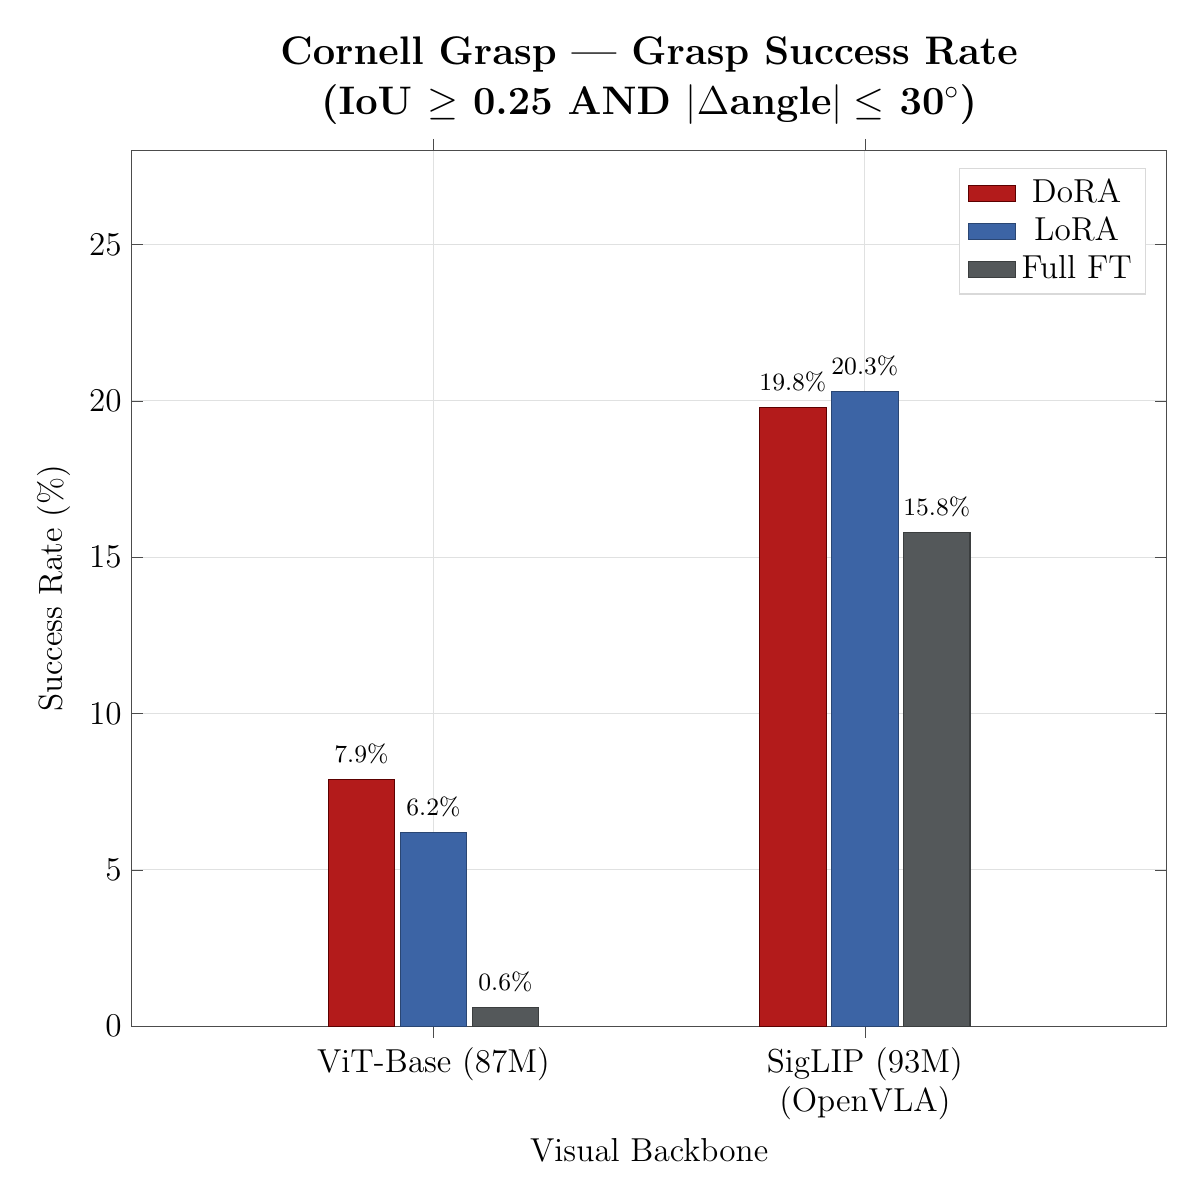
\begin{tikzpicture}
\begin{axis}[
    ybar,
    width=5.8in,
    height=5.0in,
    bar width=24pt,
    title={Cornell Grasp --- Grasp Success Rate\\(IoU $\geq$ 0.25 AND $|\Delta$angle$| \leq$ 30$^\circ$)},
    title style={font=\bfseries\Large, align=center},
    xlabel={Visual Backbone},
    ylabel={Success Rate (\%)},
    label style={font=\large},
    symbolic x coords={ViT-Base (87M),{SigLIP (93M)\\(OpenVLA)}},
    xtick=data,
    tick label style={font=\large, align=center},
    ymin=0,
    ymax=28,
    ytick={0,5,10,15,20,25},
    enlarge x limits=0.7,
    grid=major,
    major grid style={draw=CornellGray!18},
    axis line style={draw=black!70},
    tick style={draw=black!70},
    legend style={
        at={(0.98,0.98)},
        anchor=north east,
        draw=black!15,
        fill=BodyBg,
        font=\large
    },
    area legend,
    nodes near coords,
    every node near coord/.append style={
        font=\small,
        color=black,
        yshift=2pt
    },
    point meta=explicit symbolic,
]

\addplot[
    fill=CornellRed,
    draw=CornellDark,
] coordinates {
    (ViT-Base (87M),7.9) [7.9\%]
    ({SigLIP (93M)\\(OpenVLA)},19.8) [19.8\%]
};
\addlegendentry{DoRA}

\addplot[
    fill=LoRABlue,
    draw=LoRABlue!70!black,
] coordinates {
    (ViT-Base (87M),6.2) [6.2\%]
    ({SigLIP (93M)\\(OpenVLA)},20.3) [20.3\%]
};
\addlegendentry{LoRA}

\addplot[
    fill=CornellGray,
    draw=CornellGray!70!black,
] coordinates {
    (ViT-Base (87M),0.6) [0.6\%]
    ({SigLIP (93M)\\(OpenVLA)},15.8) [15.8\%]
};
\addlegendentry{Full FT}

\end{axis}
\end{tikzpicture}
\end{document}
